
\documentclass[main.tex]{subfiles}

\begin{document}
\chapter{Experiment}
\label{ch:exp}
Följande avsnitt beskriver det experiment som utfördes för att undersöka filtrenas påverkan. Vi beskriver först mätuppställningen och sedan vilka mätserier som utförts.



\section{Mätuppställning}
Mätuppställningen är baserad på \figref{fig:matuppstallning}, där våra filter placerats på vardera sida om provlådan.

\begin{comment}
\begin{figure}
    \centering
    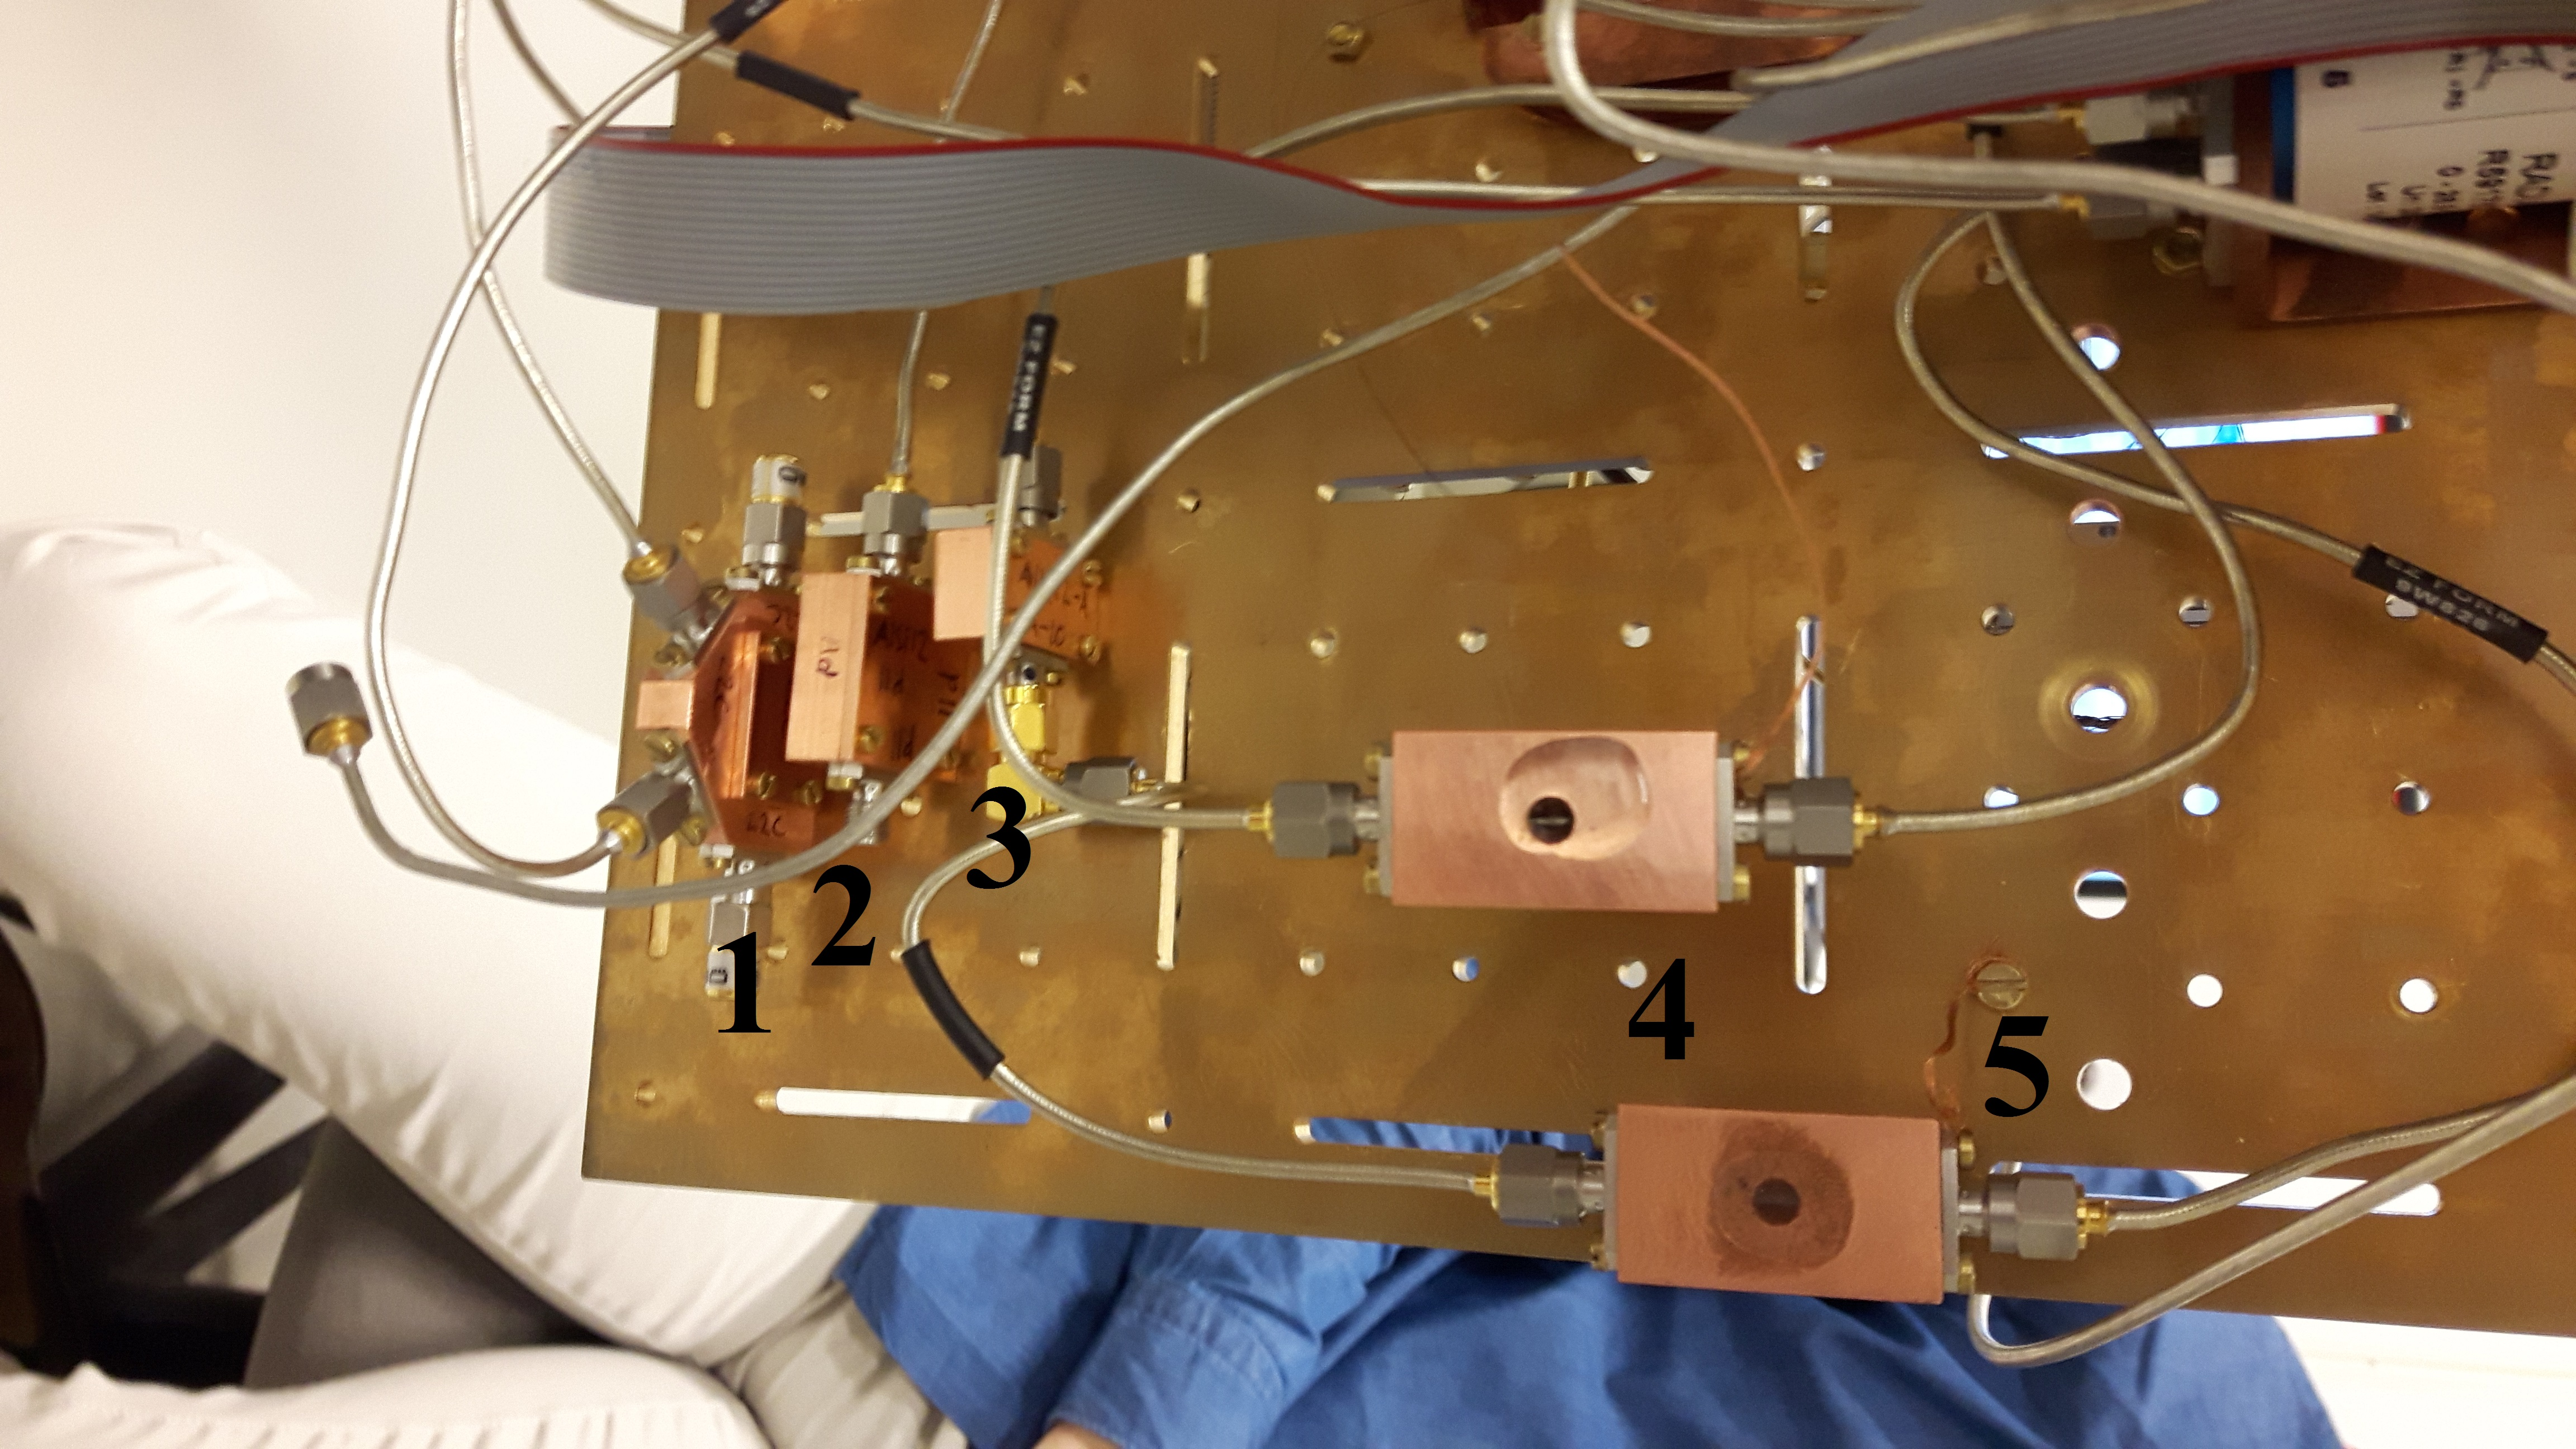
\includegraphics[scale=0.08,trim={35cm 8cm 20cm  20cm},clip]{figure/Experiment/siffroruppst.jpg}
    \caption{I figuren visas provlådorna 1,2 och 3. Till provlåda AlSi12-A är filtren med 1,895 cm respektive 1,825 cm frilagd ledare placerade (4). Filtren är kopplade till plattan med en koppartråd (5).}
    \label{fig:sifferupp}
\end{figure}
\end{comment}


\begin{comment}
\begin{figure}[h!]
    \centering
    \begin{tikzpicture}
        \node[anchor=south west,inner sep=0] (image) at (3,0) {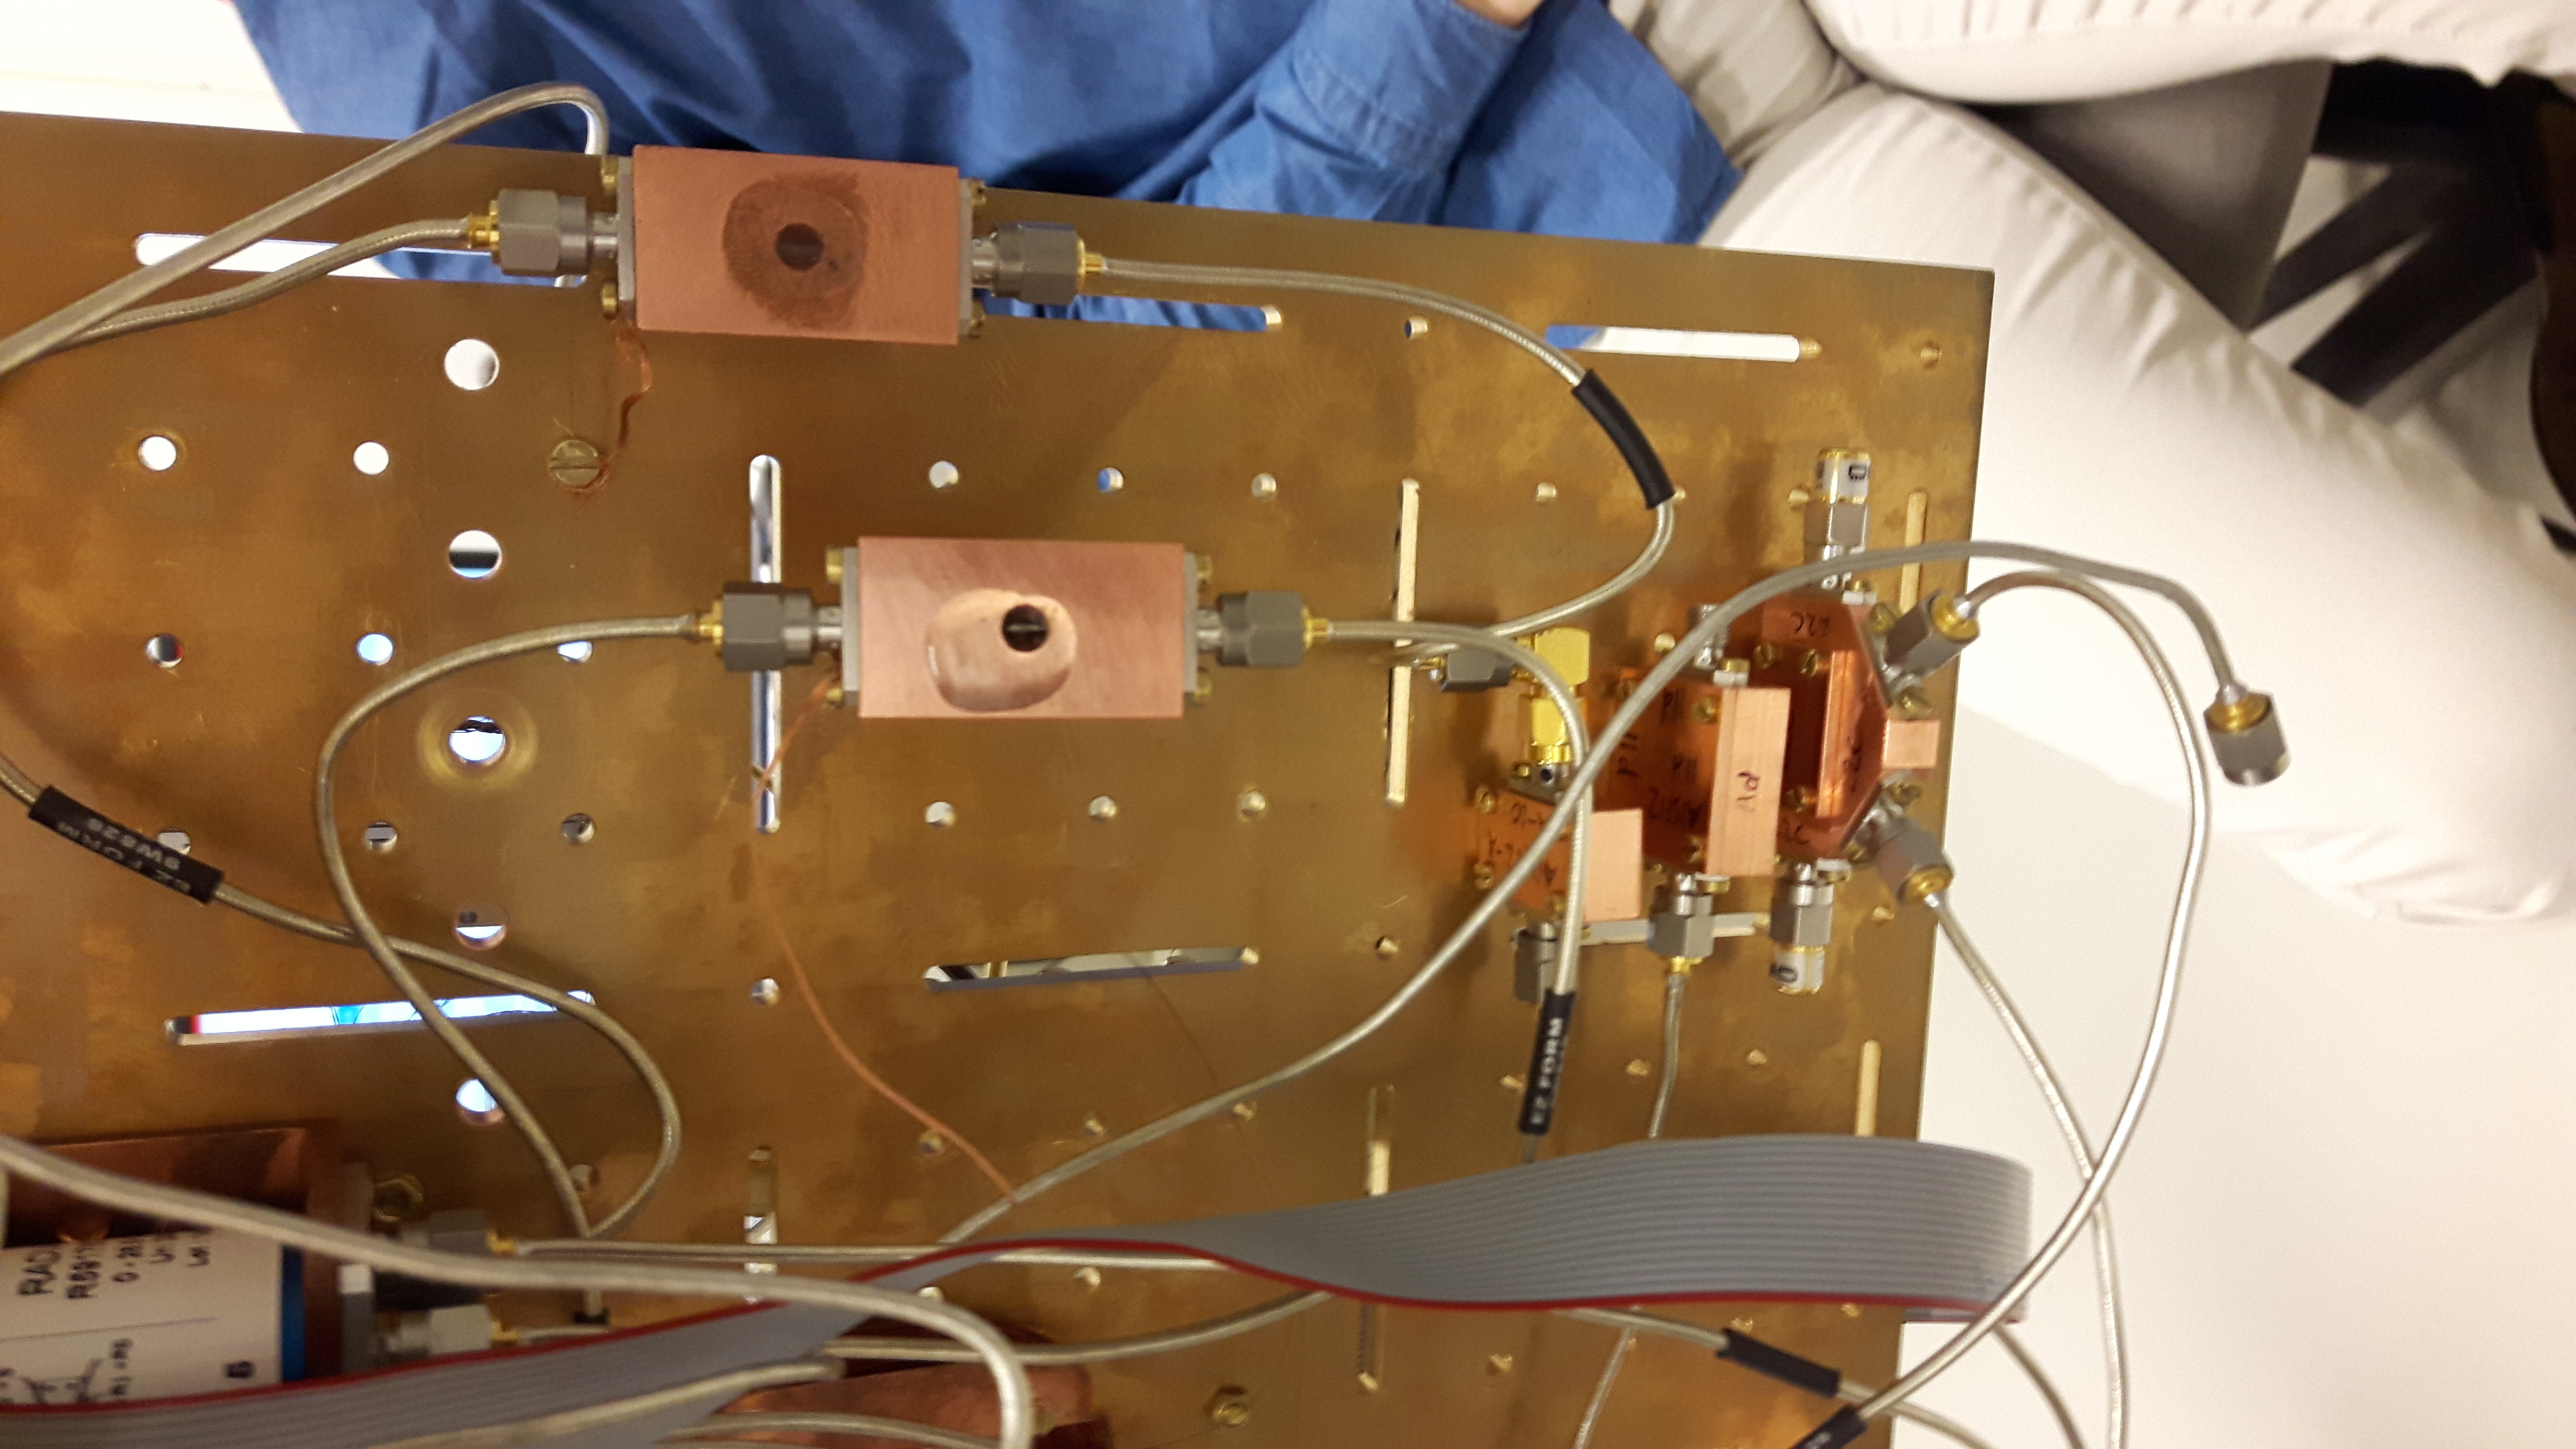
\includegraphics[width=0.1\textwidth,angle=180,trim=400 500 400 225,clip,width=0.6\linewidth]{figure/Experiment/uppstt.jpg}};
        \begin{scope}[x={(image.south east)},y={(image.north west)}]
        \node [anchor=west] at (0.3,0.4) {\Large\textbf 1};
        \node [anchor=west] at (0.34,0.4) {\Large\textbf 2};
        \node [anchor=west] at (0.4,0.45) {\Large\textbf 3};
        \node [anchor=west] at (0.65,0.3) {\Large\textbf 4};
        \node [anchor=west] at (0.8,0.35) {\Large\textbf 5};
        %\node [anchor=west] at (0.3,0.7) {\Large\textbf F};
        %\node [anchor=west] at (0.6,0.8) {\Large\textbf G};
        %\node [anchor=west] at (0.7,0.6) {\Large\textbf H};
        %\node [anchor=west] at (0.9,0.4) {\Large\textbf I};
        \end{scope}
    \end{tikzpicture}
    \caption{I figuren visas provlådorna AlSi12-22C (1), AlSi12-11d (2), och AlSi12-A (3). I figuren är filtren med 1,895 cm respektive 1,825 cm frilagd ledare kopplade till provlåda AlSi12-A  (4). Filtren är även kopplade till plattan med en koppartråd (5).}
    \label{fig:sifferupp}
\end{figure}
\end{comment}


I experimentet användes de filter som presenterats i tabell \ref{tab:filter_list}, till varje provlåda placerades två filter med ungefär lika lång frilagd ledare, ett filter innan och ett efter. Till provlåda 1 var de långa filtren kopplade, till provlåda 2 var de medellånga filtren kopplade och till provlåda 3 var de korta filtren kopplade. En koppartråd fästes även från varje filter till den guldpläterade kopparplatta som provlådorna var fästa vid. Detta gjordes för att uppnå termisk jämvikt och för att försäkra oss om att filtren kyldes ned till \unit[10]{mK}, detta eftersom värmeledningen i koaxial-kablarna kunde vara otillräcklig. % Tre filter, alla av olika längd, placerades även vid egna ingångar, för att utnyttja dessa som referenser vid låg temperatur. 


\section{Mätserier}


De olika provlådorna hade mellan nio och sex resonatorer var. För mätningarna användes centerfrekvenser som låg nära resonatorernas resonansfrekvenser, där man med ett intervall på \unit[3]{MHz} kunde se hela karakteristiken för resonatorn. Centerfrekvenserna valdes så att man fick en bra överblick över karakteristiken, både över magnitudspekrumen och fasspektrumen. Centerfrekvenserna som användes för att analysera resonatorerna visas i tabell \ref{tab:utanfil}. 

\begin{table}[h]
    \centering
        \caption{Centerfrekvenser för resonatorerna i de olika provlådorna}
    \label{tab:utanfil}
    \begin{tabular}{lccccccccc}
    \toprule
        \textbf{Provlåda}  & \multicolumn{7}{c}{Centerfrekvenser (GHz)} \\
        \midrule
        1 & 5,15 & 5,37 & 6,13 & 6,44 & 7,57 & 7,84 &\\
        2 & 4,82 & 5,01 & 5,73 & 6,02 & 7,08  &  7,32 & \\
        3 & 4,95 & 5,01 & 5,22 & 5,69 & 5,96 & 6,25 & 6,95 & 7,35 & 7,62\\
        \bottomrule
    \end{tabular}
\end{table}

%En VNA av model Agilent E8364b användes för att svepa över ett frekvensspann mellan 2 och 8 GHz, detta för att finna de olika frekvenserna för resonatorerna. I provlåda A fanns nio resonatorer och i provlådorna C och d fanns sex stycken. Signalen från ett intervall på \unit[3]{MHz} kring centerfrekvenserna analyserades sedan där värdet på ineffekten varierades.

\begin{wrapfigure}{r}{0.3\textwidth}
    \centering
    \setlength\figurewidth{0.45\linewidth}
    \setlength\figureheight{7em}
    % This file was created by matlab2tikz.
%
\definecolor{mycolor1}{rgb}{0.00000,0.44700,0.74100}%
%
\begin{tikzpicture}[%
trim axis left, trim axis right
]

\begin{axis}[%
width=\figurewidth,
height=\figureheight,
at={(0\figurewidth,0\figureheight)},
scale only axis,
xmin=-85,
xmax=-45,
xlabel style={font=\color{white!15!black}},
xlabel={Ineffekt (dBm)},
ymin=0,
ymax=250,
ylabel style={font=\color{white!15!black}},
ylabel={Medelvärdesbildningar},
axis background/.style={fill=white},
axis x line*=bottom,
axis y line*=left
]
\addplot [color=mycolor1, forget plot]
  table[row sep=crcr]{%
-83	240\\
-73	130\\
-63	35\\
-53	20\\
-48	15\\
};
\addplot [color=mycolor1, draw=none, mark=square, mark options={solid, mycolor1}, forget plot]
  table[row sep=crcr]{%
-83	240\\
-80.5	212.5\\
-78	185\\
-75.5	157.5\\
-73	130\\
-70.5	106.25\\
-68	82.5\\
-65.5	58.75\\
-63	35\\
-60.5	31.25\\
-58	27.5\\
-55.5	23.75\\
-53	20\\
-50.5	17.5\\
-48	15\\
};
\end{axis}
\end{tikzpicture}%
    \caption{Antal medelvärdesbildningar av VNA:n mot ineffekt}
    \label{fig:medel}
\end{wrapfigure}

Transmissionskoefficienterna för intervallet av frekvenser analyserades för ineffekter mellan \unit[8]{dBm} och \unit[-83]{dBm}. Eftersom VNA:n hade en övre och undre ineffekt på \unit[8]{dBm} respektive \unit[-27]{dBm} genomfördes mätningarna i 3 omgångar, där en dämpning lades till på input-kapel mellan varje omgång. Mätningarna genomfördes med en steglängd på \unit[2,5]{dBm} och varierande medelvärdesbildnignar. 

Den första mätningen gjordes utan någon dämpning i intervallet \unit[8]{dBm} till \unit[-27]{dBm}. Mätningen krävde enbart 5 medelvärdesbildningar eftersom bruset i förhållande till signalen är mycket lägre vid hög effekt.

Vid andra mätningen lades en dämpning på \unit[30]{dBm} till genom att seriekoppla en dämpare med \unit[20]{dBm} dämpning och en dämpare med \unit[10]{dBm} dämpning. Denna mätning gav data för effekter mellan \unit[-22]{dBm} och \unit[-52]{dBm}. Här krävdes det fler medelvärdesbildningar än tidigare på grund av den lägre signalen, vi använde oss av 32 stycken medelvärdesbildnignar. 

Vid tredje mätningen placerades en dämpning på totalt \unit[56]{dBm} genom att seriekoppla dämpare med dämpningar på 30,20 och \unit[6]{dBm}. Detta gav data för effekter mellan \unit[-44]{dBm} och \unit[-83]{dBm}. För denna mätning krävdes många fler medelvärdesbildningar eftersom signalen var väldigt låg i relation till  bruset. Antal medelvärdesbildningar som behövdes vid varje effekt visas i en graf i \figref{fig:medel}.

Från mätningarna ovan extrahetades datan för $S_{21}$ Med hjälp av anpassningen i avsnitt \ref{sec:anpass} kunde $Q_i$ beräknas.



%%%%%%%%%%%% BORTKOMMENTERAD SKIT %%%%%%%%%%%%

\begin{comment}
\begin{table}[h]
\centering
\begin{tabular}{|c|c|c|c|}\hline
     Switch & Sample & Filter & Batch på filter (före,efter) \\\hline
     1 & A & Short & (1,3) \\\hline
     2 & d & Medium & (1,3) \\\hline
     3 & & Short & (2) \\\hline
     4 & C & Long & (1,3) \\\hline
     5 & & Long & (2) \\\hline
     6 & & Medium & (2) \\\hline
\end{tabular}
\end{table}

\end{comment}

%\section{Parametrar från modellanpassningen}


\end{document}
